% ============================================================================
% ЧАСТЬ 1. Система радиочастотной идентификации
% ============================================================================
\section{Распределенная система радиочастотной идентификации транспорта}
\begin{frame}[plain, noframenumbering]
    \begin{center}
        \Huge
        Распределенная система радиочастотной идентификации транспорта
    \end{center}
\end{frame}

\begin{frame}
    \frametitle{Система радиочастотной идентификации}
    \begin{center}
    % \vfill
    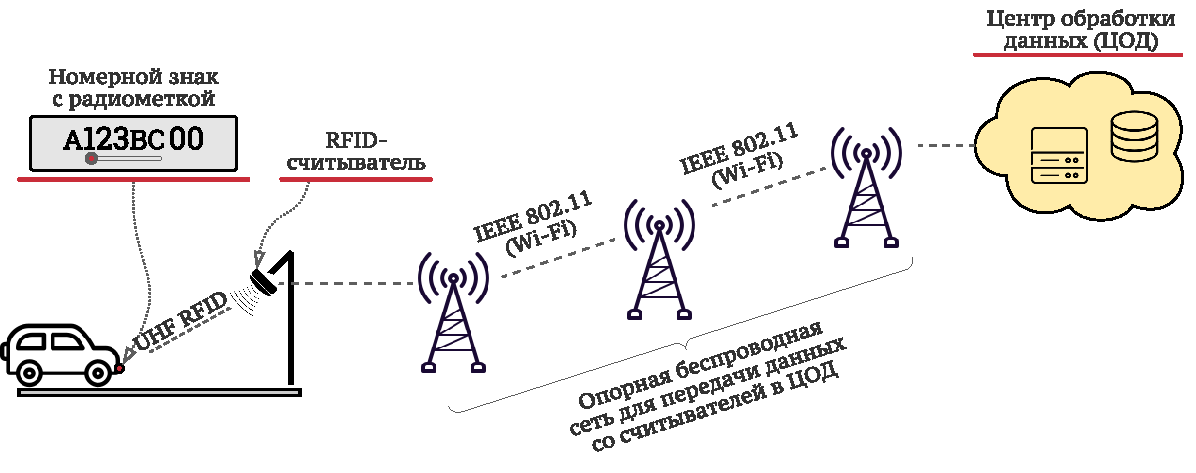
\includegraphics[width=0.9\linewidth]{chapter1/ch1_system_overview}
    \end{center}

    Система радиочастотной идентификации транспорта предназначена для
    идентификации транспорта с помощью размещенных на машинах RFID-меток
    и передачи данных по сети в центр обработки данных. Области применения:
    \begin{itemize}
        \item Повышение безопасности на дорогах "--- надежная идентификация нарушителей, поиск угнанных автомобилей
        \item Бесконтактная оплата проезда по платным дорогам
        \item Контроль доступа, оплата парковки и другие применения
    \end{itemize}
    \vfill
\end{frame}
\note{
    Этот текст будет виден только если его отображение включено
    в~файле \textbf{Presentation/setup}.
    Для раздельного вывода презентации и заметок на~разные экраны (как
    в~impress или powerpoint) можно использовать программу
    \textit{pdf-presenter-console}.
}

\begin{frame}
    \frametitle{Компоненты системы радиочастотной идентификации}
    \begin{enumerate}
        \item Радиометки
        \item RFID-считыватели
        \item Сеть передачи данных
        \item Центр обработки данных
    \end{enumerate}
\end{frame}

\begin{frame}[allowframebreaks]
    \frametitle{Постановка задач исследования}
    Для эффективного использования UHF RFID для идентификации движущихся машин были решены следующие задачи:
    \begin{enumerate}
        \item Выявить факторы, влияющие на вероятность успешной идентификации мобильной RFID-метки.
        \item Построить формальную математическую модель системы радиочастотной идентификации, исследовать свойства операций, осуществляемых считывателем над множеством мобильных меток.
        \item Разработать аналитические и имитационные модели для получения оценки вероятности идентификации мобильных RFID-меток.
        \item Определить параметры протокола, при которых доля успешно идентифицированных автомобилей с RFID-метками оказывается не ниже 90\%.
    \end{enumerate}
    \framebreak
    Для оценки производительности беспроводной сети были решены следующие задачи:
    \begin{enumerate}
        \item Поиск PH-распределений, адекватно моделирующих время обслуживания в беспроводных сетях с каналами CSMA/CA.
        \item Оценка возможности использования метода аппроксимации выходящих потоков для получения численных оценок межконцевых задержек в открытых тандемных сетях массового обслуживания с узлами типа MAP/PH/1/N.
        \item Получение численных оценок межконецвых задержек для многошаговой беспроводной сети с помощью аналитического и имитационного моделирования.
    \end{enumerate}
    \framebreak
    Для экспериментального исследования производительности системы радиочастотной идентификации были решены следующие задачи:
    \begin{enumerate}
        \item Разработка архитектуры распределённой системы управления RFID-считывателями и протоколов связи между компонентами системы.
        \item Программная реализация распределённой системы управления и разработка программного обеспечения для приема, обработки и записи данных о прочитанных метках.
        \item Проведение экспериментальных исследований и получение оценки вероятности успешной идентификации автомобилей при различных скоростях движения, маневрах, погодных условиях.
    \end{enumerate}
\end{frame}
\note[itemize]{
    \item Тезис 1
    \item Тезис 2
    \item Тезис 3
}


% ============================================================================
% ЧАСТЬ 2. ИССЛЕДОВАНИЕ ПРОИЗВОДИТЕЛЬНОСТИ СИСТЕМ РАДИОЧАСТОТНОЙ ИДЕНТИФИКАЦИИ
% ============================================================================
\section{Исследование производительности систем радиочастотной идентификации}
\begin{frame}[plain, noframenumbering]
    \begin{center}
        \Huge
        Исследование производительности систем радиочастотной идентификации
    \end{center}
\end{frame}

\begin{frame}
    \frametitle{Структура системы}
\end{frame}


\begin{frame}
    \frametitle{Моделирование радиоканала}
\end{frame}

\begin{frame}
    \frametitle{Расчет BER}
\end{frame}


\begin{frame}
    \frametitle{Длительности команд и ответов}
\end{frame}

\begin{frame}
    \frametitle{Результаты: число раундов}
\end{frame}

\begin{frame}[allowframebreaks]
    \frametitle{Результаты: вероятность идентификации}
\end{frame}

\begin{frame}
    \frametitle{Выводы}
\end{frame}



% ============================================================================
% ЧАСТЬ 3. АНАЛИТИЧЕСКАЯ МОДЕЛЬ СИСТЕМЫ РАДИОЧАСТОТНОЙ ИДЕНТИФИКАЦИИ
% ============================================================================
\section{Аналитическая модель системы радиочастотной идентификации}
\begin{frame}[plain, noframenumbering]
    \begin{center}
        \Huge
        Аналитическая модель системы радиочастотной идентификации
    \end{center}
\end{frame}

\begin{frame}
    \frametitle{Сбросы питания считывателя и флаги сессий в RFID}
\end{frame}

\begin{frame}
    \frametitle{Ограничения и допущения модели}
\end{frame}

\begin{frame}
    \frametitle{Постановка задачи}
\end{frame}

\begin{frame}
    \frametitle{Моделирование раундов инвентаризации}
\end{frame}

\begin{frame}
    \frametitle{Элементарные операции}
\end{frame}

\begin{frame}
    \frametitle{Размеченные сценарии}
\end{frame}

\begin{frame}
    \frametitle{Определение фонового процесса}
\end{frame}

\begin{frame}
    \frametitle{Матрицы операций фнового процесса}
\end{frame}

\begin{frame}
    \frametitle{Расчет распределения числа активных меток}
\end{frame}

\begin{frame}
    \frametitle{Определение основного процесса}
\end{frame}

\begin{frame}
    \frametitle{Матрицы операций основного процесса}
\end{frame}

\begin{frame}
    \frametitle{Расчет вероятности идентификации}
\end{frame}

\begin{frame}
    \frametitle{Результаты: анализ свойств раундов}
\end{frame}

\begin{frame}
    \frametitle{Результаты: валидация модели}
\end{frame}

\begin{frame}
    \frametitle{Результаты: вероятность идентификации}
\end{frame}

\begin{frame}
    \frametitle{Выводы}
\end{frame}





% ============================================================================
% ЧАСТЬ 4. АНАЛИЗ ПРОИЗВОДИТЕЛЬНОСТИ ОПОРНОЙ БЕСПРОВОДНОЙ СЕТИ
% ============================================================================
\section{Анализ производительности опорной беспроводной сети}
\begin{frame}[plain, noframenumbering]
    \begin{center}
        \Huge
        Анализ производительности опорной беспроводной сети
    \end{center}
\end{frame}

\begin{frame}
    \frametitle{Беспроводная сеть передачи данных}
\end{frame}

\begin{frame}
    \frametitle{Моделирование беспроводной сети с помощью СеМО}
\end{frame}

\begin{frame}
    \frametitle{PH-распределения}
\end{frame}

\begin{frame}
    \frametitle{MAP-потоки}
\end{frame}

\begin{frame}
    \frametitle{Многофазные сети с узлами MAP/PH/1/N}
\end{frame}

\begin{frame}
    \frametitle{Итерационный расчет характеристик СеМО}
\end{frame}

\begin{frame}
    \frametitle{Расчет характеристик СеМО методом Монте-Карло}
\end{frame}

\begin{frame}
    \frametitle{Расчет методом понижения размерностей потоков}
\end{frame}

\begin{frame}
    \frametitle{Набор денных для проведения численных исследований}
\end{frame}

\begin{frame}
    \frametitle{Аппроксимация потоков по среднему значению}
\end{frame}

\begin{frame}
    \frametitle{Аппроксимация PH по двум моментам}
\end{frame}

\begin{frame}
    \frametitle{Аппроксимация PH по трем моментам}
\end{frame}

\begin{frame}
    \frametitle{Аппроксимация MAP по трем моментам и корреляции}
\end{frame}

\begin{frame}
    \frametitle{Сравнение эффективности методов аппроксимации}
\end{frame}

\begin{frame}
    \frametitle{Длительность передачи пакета в IEEE 802.11}
\end{frame}

\begin{frame}
    \frametitle{Калибровочная беспроводная сеть}
\end{frame}

\begin{frame}
    \frametitle{Методика: выбор PH-распределений для модели сети}
\end{frame}

\begin{frame}
    \frametitle{Имитационное моделирование беспроводной сети}
\end{frame}

\begin{frame}
    \frametitle{Характеристики каналов калибровочной сети}
\end{frame}

\begin{frame}
    \frametitle{Валидация модели по калибровочной сети}
\end{frame}

\begin{frame}
    \frametitle{Межконцевые задержки в сетях проивзольного размера}
\end{frame}

\begin{frame}
    \frametitle{Изменение задержек в каналах}
\end{frame}

\begin{frame}
    \frametitle{Обновленная методика выбора распределений}
\end{frame}

\begin{frame}
    \frametitle{Межконцевые задержки (обновленная методика)}
\end{frame}

\begin{frame}
    \frametitle{Ошибки в оценке задержек}
\end{frame}

\begin{frame}
    \frametitle{Выводы}
\end{frame}


% ============================================================================
% ЧАСТЬ 5. РАЗРАБОТКА И ЭКСПЕРИМЕНТАЛЬНОЕ ВНЕДРЕНИЕ СИСТЕМЫ РАДИОЧАСТОТНОЙ
%          ИДЕНТИФИКАЦИИ
% ============================================================================
\section{Разработка и экспериментальное внедрение системы радиочастотной идентификации}
\begin{frame}[plain, noframenumbering]
    \begin{center}
        \Huge
        Разработка и экспериментальное внедрение системы радиочастотной идентификации
    \end{center}
\end{frame}

\begin{frame}
    \frametitle{Постановка задачи}
\end{frame}

\begin{frame}
    \frametitle{Архитектура распределенной системы}
\end{frame}

\begin{frame}
    \frametitle{Основные компоненты системы}
\end{frame}

\begin{frame}
    \frametitle{Способы размещения компонентов}
\end{frame}

\begin{frame}
    \frametitle{Протоколы связи между компонентами}
\end{frame}

\begin{frame}
    \frametitle{Протокол управления компонентами IMMP}
\end{frame}

\begin{frame}
    \frametitle{Протокол работы с RFID-адаптерами ITOP}
\end{frame}

\begin{frame}
    \frametitle{Протокол подключения абонентов TFP}
\end{frame}

\begin{frame}
    \frametitle{Протокол подключения интерфейсов SUAP}
\end{frame}

\begin{frame}
    \frametitle{Организация параллельной обработки}
\end{frame}

\begin{frame}
    \frametitle{Особенности реализации системы}
\end{frame}

\begin{frame}
    \frametitle{Структура RFID-считывателя}
\end{frame}

\begin{frame}
    \frametitle{Эксперимент №1: Казань, 2014 год}
\end{frame}

\begin{frame}
    \frametitle{Эксперимент №2: Казань, 2020 год}
\end{frame}

\begin{frame}
    \frametitle{Эксперимент №3: ЦКАД, 2021 год}
\end{frame}

\begin{frame}
    \frametitle{Выводы}
\end{frame}

% % ============================================================================
% % ЧАСТЬ 6. ЗАКЛЮЧЕНИЕ
% % ============================================================================
% \section{Заключение}



% ============================================================================
% ЧАСТЬ -. ПРИМЕРЫ
% ============================================================================
\section{-- Примеры --}
\begin{frame}[plain, noframenumbering]
    \begin{center}
        \Huge
        ПРИМЕРЫ ИЗ ПАКЕТА PHD-THESIS-LATEX
    \end{center}
\end{frame}
\begin{frame}[plain, noframenumbering]
    \begin{center}
        \Huge
        Графика
    \end{center}
\end{frame}


\begin{frame}[plain, noframenumbering]
    \frametitle{Одиночное изображение}
    \centering
    \includegraphics[width=0.8\linewidth]{latex} % окружение figure не требуется
\end{frame}

\begin{frame}[plain, noframenumbering]
    \frametitle{Векторная графика}
    \begin{figure}
	    \centering
	    \ifdefmacro{\tikzsetnextfilename}{\tikzsetnextfilename{tikz_presentation}}{}% присваиваемое предкомпилированному pdf имя файла (не обязательно)
	    \input{Presentation/images/tikz_plot.tikz}
    \end{figure}
\end{frame}


\begin{frame}[plain, noframenumbering]
    \frametitle{Изображения по-вертикали}
    \centering
    \vfill
    \includegraphics[width=0.8\linewidth,height=0.1\textheight]{latex} \\
    \TeX
    \vfill
    \includegraphics[width=0.8\linewidth,height=0.2\textheight]{latex} \\
    \LaTeX
    \vfill
    \includegraphics[scale=0.2]{latex} \\
    \vfill
\end{frame}


\begin{frame}[plain, noframenumbering]
    \frametitle{Изображения по-горизонтали}
    \begin{minipage}[t]{0.47\linewidth}
        \textbf{Составная \\ подпись 1}
        \center{\includegraphics[width=1\linewidth]{knuth1}}
    \end{minipage}
    \hfill
    \begin{minipage}[t]{0.47\linewidth}
        \textbf{Составная \\ подпись 2}
        \center{\includegraphics[width=1\linewidth]{knuth2}}
    \end{minipage}
\end{frame}

\begin{frame}[plain, noframenumbering]
    \frametitle{Разделяющие линии}
    \begin{minipage}[c]{0.47\linewidth}
        \center{\includegraphics[width=1\linewidth]{latex}}
        \bigskip
        \hrule{}
        \bigskip
        \textbf{Составная \\ подпись 1}
    \end{minipage}
    \hfill
    \vrule{}
    \hfill
    \begin{minipage}[c]{0.47\linewidth}
        \flushright
        \textbf{Составная \\ подпись 2}
        \center{\includegraphics[width=1\linewidth]{knuth2}}
    \end{minipage}
\end{frame}

\begin{frame}[plain, noframenumbering]
    \begin{center}
        \Huge
        Остальное
    \end{center}
\end{frame}


\begin{frame}[plain, noframenumbering]
    \frametitle{Формулы}
    \[
    \left\{
    \begin{array}{rl}
        \dot x = & \sigma (y-x)  \\
        \dot y = & x (r - z) - y \\
        \dot z = & xy - bz
    \end{array}
    \right.
    \]
\end{frame}

\begin{frame}[plain, noframenumbering]
    \frametitle{amsmath}
    \centering
    \begin{minipage}[t]{0.5\linewidth}
        \begin{multline*}
            y = 1 x^1 + 2 x^2 + 3 x^3 + \\ + 4 x^4 + 5 x^5 + \dots
        \end{multline*}
    \end{minipage}
\end{frame}

\begin{frame}[allowframebreaks, noframenumbering]
    \frametitle{Уравнения Максвелла}
    \centering{
        \small
        \def\arraystretch{1.8}%
        \begin{tabular}{ll}
            \toprule
            Интегральная форма                                                                                                                                          & Дифференциальная форма                                                        \\ \midrule
            \(Q_e(t) = \displaystyle\oiint_S \vec D(t) \cdot d\vec{s} = \displaystyle\iiint_V \rho_v(t) dv\)                                                              & \(\nabla \cdot \vec D(t) = \rho_v(t)\)                                          \\
            \(\displaystyle\oiint_S \vec B(t) \cdot d\vec{s} = 0\)                                                                                                        & \(\nabla \cdot \vec B(t) = 0\)                                                  \\
            \(V_{emf}(t) = \displaystyle\oint_L \vec E(t) \cdot d\vec{l}\) = \(- \displaystyle\iint_S \left[\frac{\partial\vec{B}(t)}{\partial t}\right] \cdot d\vec{s}\)   & \(\nabla \times \vec E(t) = - \frac{\partial\vec{B}(t)}{\partial t}\)           \\
            \(I(t) = \displaystyle\oint_L \vec H(t) \cdot d\vec{l} = \displaystyle\iint_S \left[\vec J(t) + \frac{\partial\vec{D}(t)}{\partial t}\right] \cdot d\vec{s}\) & \(\nabla \times \vec H(t) = \vec J(t) + \frac{\partial\vec{D}(t)}{\partial t}\) \\ \midrule
            \(\displaystyle\oiint_S \vec J \cdot d\vec{s} = -\frac{\partial Q_e}{\partial t}\)                                                                            & \(\nabla \cdot \vec J = - \frac{\partial \rho_v}{\partial t}\)                  \\
            \bottomrule
            \multicolumn{2}{c}{\(\vec D(t) = \left[\varepsilon(t)\right] * \vec E(t)\)}                                                                                                                                                                   \\
            \multicolumn{2}{c}{\(\vec B(t) = \left[\mu(t)\right] * \vec H(t)\)}                                                                                                                                                                           \\
        \end{tabular}
    }
    \framebreak

    \hspace{0.05\linewidth}
    \centering{
        \small
        \def\arraystretch{1.8}%
        \begin{tabular}{ll}
            \toprule
            Интегральная форма                                                                                                            & Дифференциальная форма                             \\ \midrule
            \(Q_e = \displaystyle\oiint_S \vec D \cdot d\vec{s} = \displaystyle\iiint_V \rho_v dv\)                                         & \(\nabla \cdot \vec D = \rho_v\)                     \\
            \(\displaystyle\oiint_S \vec B \cdot d\vec{s} = 0\)                                                                             & \(\nabla \cdot \vec B = 0\)                          \\
            \(V_{emf} = \displaystyle\oint_L \vec E \cdot d\vec{l}\) = \(- \displaystyle\iint_S \left[j \omega \vec B\right] \cdot d\vec{s}\) & \(\nabla \times \vec E = - j \omega \vec B\)         \\
            \(I = \displaystyle\oint_L \vec H \cdot d\vec{l} = \displaystyle\iint_S \left[\vec J + j \omega \vec D\right] \cdot d\vec{s}\)  & \(\nabla \times \vec H = \vec J + j \omega \vec{D}\) \\ \midrule
            \(\displaystyle\oiint_S \vec J \cdot d\vec{s} = - j \omega Q_e\)                                                                & \(\nabla \cdot \vec J = - j \omega \rho_v\)          \\
            \bottomrule
            \multicolumn{2}{c}{\(\vec D(t) = \left[\varepsilon\right] \vec E(t)\)}                                                                                                               \\
            \multicolumn{2}{c}{\(\vec B(t) = \left[\mu\right] \vec H(t)\)}                                                                                                                       \\
        \end{tabular}
    }
\end{frame}

\begin{frame}[plain, noframenumbering]
    \frametitle{Таблица}
    \centering
    \begin{tabular}{|l|l|}
        \hline
        \textbf{Заголовок 1} & \textbf{Заголовок 2} \\
        \hline
        Сумма                & \(b+a\)                \\
        \hline
        Разность             & \(a-b\)                \\
        \hline
        Произведение         & \(a*b\)                \\
        \hline
    \end{tabular}
\end{frame}

\begin{frame}[plain, noframenumbering]
    \frametitle{Другая таблица}
    \centering
    \begin{tabular}{lc}
        \toprule
        \multicolumn{1}{c}{\textbf{Заголовок 1}} & \textbf{Заголовок 2} \\ \midrule
        Сумма                                    & \(b+a\)                \\
        Разность                                 & \(a-b\)                \\
        Произведение                             & \(a*b\)                \\
        \bottomrule
    \end{tabular}
\end{frame}


\begin{frame}[plain, noframenumbering]
    \frametitle{Большой многоуровневый список}
    \begin{itemize}
        \item \textbf{Пункт 1}
              \begin{itemize}
                  \itemi Подпункт 1-1
                  \itemi Подпункт 1-2
              \end{itemize}
        \item \textbf{Пункт 2}
              \begin{itemize}
                  \itemi Подпункт 2-1
              \end{itemize}
        \item \textbf{Пункт 3}
              \begin{itemize}
                  \itemi Подпункт 3-1
                  \itemi Подпункт 3-2
              \end{itemize}
        \item \textbf{Пункт 4}
              \begin{itemize}
                  \itemi Подпункт 4-1
              \end{itemize}
        \item \textbf{Пункт 5}
              \begin{itemize}
                  \itemi Подпункт 5-1
                  \itemi Подпункт 5-2
                  \itemi Подпункт 5-3
              \end{itemize}
    \end{itemize}
\end{frame}

\begin{frame}[plain, noframenumbering]
    \frametitle{Четыре изображения}
    \centering
    \includegraphics[width=0.35\linewidth,angle=35]{latex}
    \includegraphics[width=0.35\linewidth,angle=135]{latex}\\
    \includegraphics[width=0.35\linewidth,angle=15]{latex}
    \includegraphics[width=0.35\linewidth,angle=-15]{latex}
\end{frame}

\begin{frame}[allowframebreaks]
    \frametitle{Списки}
    \begin{itemize}
        \item Проблема 1
        \item Проблема 2
        \item Проблема 3
    \end{itemize}
    \framebreak
    \begin{enumerate}
        \item \textbf{Задача 1}
              \begin{itemize}
                  \item Подзадача 1-1
                  \item Подзадача 1-2
              \end{itemize}
        \item \textbf{Задача 2}
              \begin{itemize}
                  \item Подзадача 2-1
                  \item Подзадача 2-2
                  \item Подзадача 2-3
              \end{itemize}
        \item \textbf{Задача 3}
              \begin{itemize}
                  \item Подзадача 3-1
                  \item Подзадача 3-2
                  \item Подзадача 3-3
              \end{itemize}
    \end{enumerate}
    \framebreak
    Поясняющий текст
    \begin{itemize}
        \item Один
        \item Два
        \item Три
    \end{itemize}
\end{frame}
\note[itemize]{
    \item Тезис 1
    \item Тезис 2
    \item Тезис 3
}
